% Source of the figure cut-path.pdf (a cut-path between u and v, schematic).
% Compile with pdfLaTeX; the PDF is included in the manuscript at its natural size.
\documentclass[tikz,border=1pt]{standalone}
\usepackage[T1]{fontenc}
\usepackage{stix}
\pdfinfoomitdate=1 \pdftrailerid{} \pdfsuppressptexinfo=-1
\definecolor{threadblue}{RGB}{31,102,178}
\definecolor{threadred}{RGB}{200,40,40}
\begin{document}
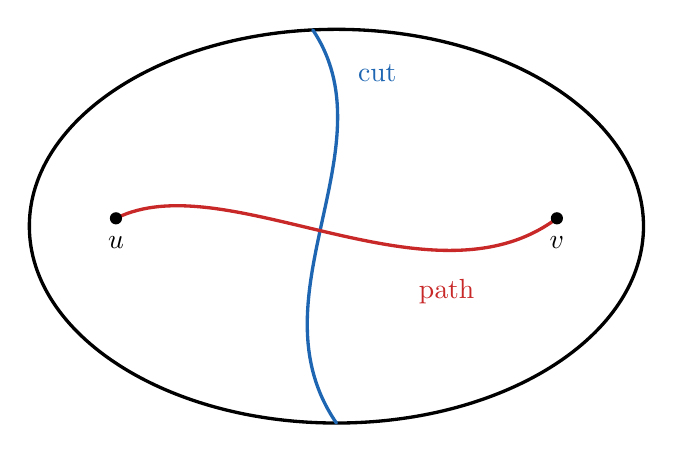
\begin{tikzpicture}[x=1cm, y=1cm,
    chain/.style={line width=1.2pt, line cap=round, line join=round}]
  % the graph
  \draw[chain] (4,2.6) ellipse[x radius=3.9, y radius=2.5];
  % the cut, from the top to the bottom of the graph
  \draw[chain, threadblue] (3.7,5.093) .. controls (4.7,3.6) and (2.9,1.7) .. (4.0,0.1);
  \node[threadblue, anchor=west] at (4.15,4.55) {cut};
  % the u-v path
  \draw[chain, threadred] (1.2,2.7) .. controls (2.6,3.4) and (5.2,1.5) .. (6.8,2.7);
  \node[threadred, anchor=north] at (5.4,2.05) {path};
  \fill (1.2,2.7) circle[radius=2.2pt] (6.8,2.7) circle[radius=2.2pt];
  \node[below=3pt] at (1.2,2.7) {$u$};
  \node[below=3pt] at (6.8,2.7) {$v$};
\end{tikzpicture}
\end{document}
